% !TEX program = XeTeX
\documentclass[12pt, aspectratio=149]{beamer}% aspectratio's: 169, 1610, 149, 54, 43 and 32
\graphicspath{{images/},
			  {logos/},
			  {MathAnimation/},
			  {../Thesis_report_Wesley/Figures/}}


% For MAC users: change the builder to LuaLaTex

% Instructions to get this template working:
%  - For windows users: install MikTex (explicitely!) as admin,
%    otherwise you get the error the error:
%    "Sorry, but "MiKTeX Compiler Driver" did not succeed."
%  - Use MiTex to install cm-super, otherwise your font may be pixxellated


% Best practices/tips:
%  - Select aspect ratio (see line 2), so you don't have black borders with your specific beamer
%
%  - Code to show side by side figures:
% 	 \begin{columns}
% 	   \column{\dimexpr\paperwidth}
% 	   \begin{figure}
% 	   	\includegraphics[width=0.46\textwidth]{image1}
%             \hspace{\dimexpr0.02\textwidth}
% 	    \includegraphics[width=0.46\textwidth]{image2}
% 	   \end{figure}
% 	 \end{columns}


% Usetheme options, see below:
% 	- titlebgimage = image on title slide. Please make
% 	  sure to crop the top or bottom if it's too tall
% 	- thankyoubgimage = image on the thank you slide
%   - External institute or company logo on title and thank you page
% 	- totalframenumber = for page numbering, an option to
%     show the total amount of frame numbers on each frame
%   - slidesperpage = option to make handouts
\usetheme[
titlebgimage      = TitleImage_Crack,
thankyoubgimage   = logos/MoM_Microscope_Cropped,
% externalimage     = logos/CompanyLogo,
totalframenumber  = true,
slidesperpage     = 1
]{phstyle}

\title    {Presentation title goes here}% Set title
\subtitle {Subtitle goes here}% Set subtitle
\author   {Firstname Lastname}% author
\institute{Mechanics of Materials}% institute (department)

\newcommand{\Committee}{% Set committee members:
Supervisors:\\
Dr. Ir. initials \& Lastname,\\
Dr. Ir. initials \& Lastname}% title slide: committee members


\begin{document}

\begin{TitleSlide}\end{TitleSlide}% Title

% Table of contents:
% 	To change item separation distance: the value between the [t]'s
% 	To change horizontal placement: change size of the parbox
%   To change vertical placement: change the vspace
	\begin{TableOfContents}
	\vspace{2mm}
	\hfill\parbox{.72\textwidth}{
	\begin{minipage}[t][4cm][t]{\textwidth}
	\tableofcontents
	\end{minipage}}
	\end{TableOfContents}

% Subjects, sorted by "chapters":
	%!TEX ROOT = ../presentation.tex

\section{Introduction}


\begin{frame}
    Items and enumerations:
    \begin{itemize}
        \item Motivation for research
        \item The phenomenon under investigation
        \begin{itemize}
            \item Relation to ... 
        \end{itemize}
    \end{itemize}
    \vspace{5mm}
    Steps:
    \begin{enumerate}
        \item Step 1
        \item Step 2
    \end{enumerate}
\end{frame}








	%!TEX ROOT = ../presentation.tex


\section{First section name}% Section for TOC slides


\begin{frame}
    \vspace{9mm}
    Figure with the source of the image as footnote:\\
    % \vspace{3mm}
    \begin{figure}[H] \begin{center}
        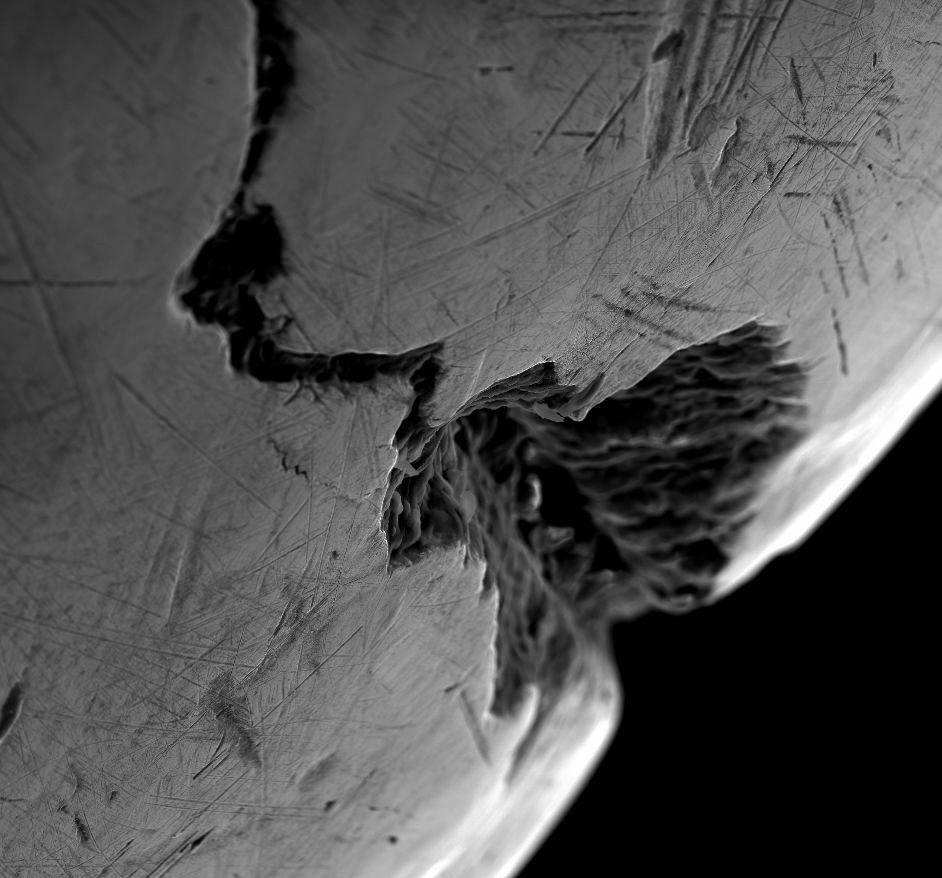
\includegraphics[height=0.7\textheight]{TitleImage_Crack}
    \end{center} \end{figure}
    \footn{Image source: Science \cite{ScienceCom}}
\end{frame}



\begin{frame}
    Side by side images from research by \cite{Web_Experiment}
    \begin{columns}
    \column{\dimexpr\paperwidth}
    \begin{figure}%
        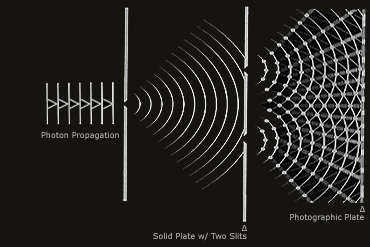
\includegraphics[height=0.4\textheight]{ExperimentalSetup}%
               \hspace{\dimexpr0.02\textwidth}%
        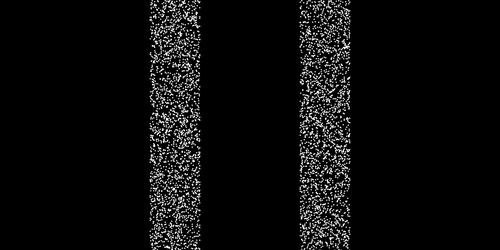
\includegraphics[height=0.4\textheight]{ExperimentalObservations}%
    \end{figure}%
    \end{columns}
    \footn{Source of images: theobservereffect.com \cite{Web_Experiment}}
\end{frame}




	%!TEX ROOT = ../presentation.tex

% \section{Name of Section two}% Section for TOC slides

% \subsection{Composition of the anode}% Optional, if you want to include subsection in TOC slides

\begin{frame}
	A sketch with IPE (click to download: \href{http://ipe.otfried.org/}{ipe.otfried.org}) \\ and a Matlab figure:
	\vspace{-4mm}
	\begin{columns}
	\column{\dimexpr\paperwidth}
	\begin{figure}%
	    
\includegraphics[width=0.24\textwidth]{Sketch_Ring}%
	           \hspace{\dimexpr0.02\textwidth}%
	    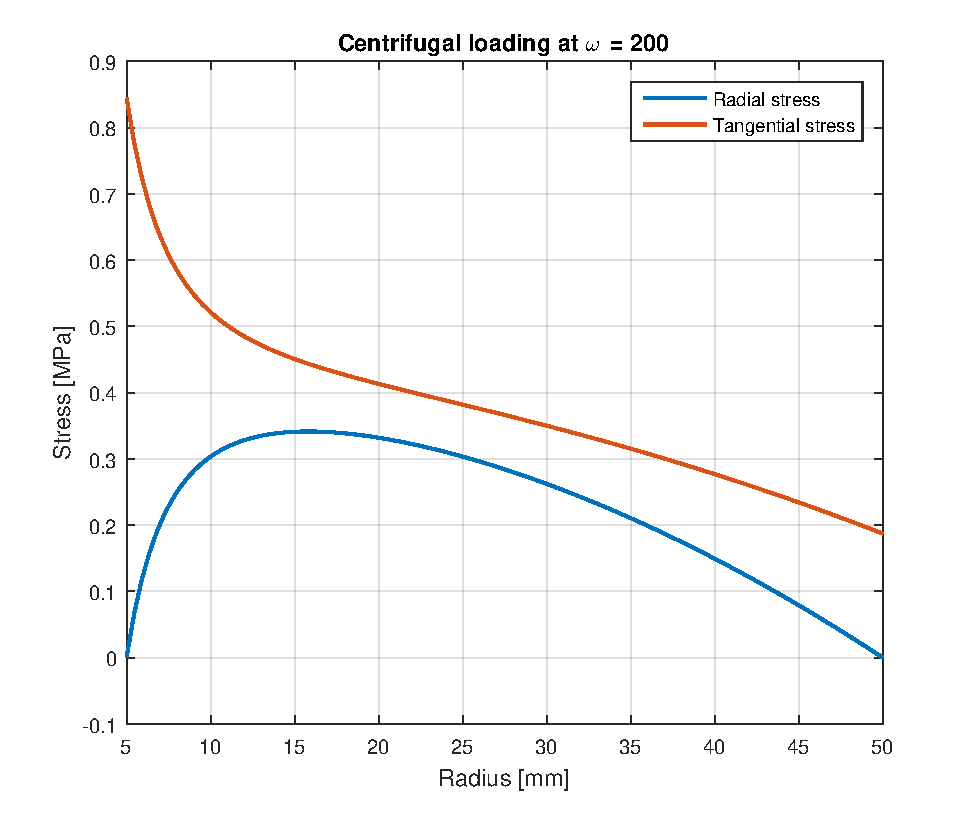
\includegraphics[width=0.5\textwidth]{Matlab_Figure}%
	\end{figure}%
	\end{columns}
\end{frame}


	%!TEX ROOT = ../presentation.tex


\section{Section with an equation}% Section for TOC slides

% \subsection{Composition of the anode}% Optional, if you want to include subsection in TOC slides

\begin{frame}
	\vspace{6mm}
	Verification of thermal radiation:
	\begin{align*}
	dE 	   ~&=  - S \,e\, A dt (T^4 - T_c^4) ~ \left[ \,J\, \right]\\
	dT     ~&= \frac{dE}{C_p\, m} ~ \left[ \,K\, \right]
	\end{align*}

\end{frame}



\section{Section with Matlab (vector) animation}% Section for TOC slides

\begin{frame}
	(commented)

	% Instructions: open "phstyle.sty" and uncomment this line: "\usepackage{animate}"
	% After uncommenting you can uncomment the code below

	% \vspace{4mm}
	% Warning: this animation will only start moving in some pdf readers (e.g. Adobe)
	% \vspace{-4mm}
	% \begin{figure}[H]
	% \begin{center}%\usepackage{animate}
	% %\animategraphics[<options>]{<fps>}{<filename>}{<first frame>}{<last frame>}
	% \animategraphics[autoplay,loop,height=0.7\textheight]{15}{MathAnimation/MyAnimation}{}{}
	% \end{center} \end{figure}
	% \footn{Source: \href{http://marchetti-engine.com/}{marchetti-engine.com}}
\end{frame}








	%!TEX ROOT = ../presentation.tex
\section{Conclusions}
\begin{frame}

	\Large% Set large font for all following text:
		Conclusions

	\normalsize% Set normal font for all following text:
		\begin{itemize}
			\setlength\itemsep{2em}
			\item Primary conclusion
			\begin{itemize}
				\item Thing 1
				\begin{itemize}
					\item Subactivity
				\end{itemize}
				\item Thing 2
				\item Thing 3
			\end{itemize}
			\item Recommendations
			\begin{itemize}
				\item Something else
				\item Something else
			\end{itemize}
		\end{itemize}
\end{frame}


\begin{References}\end{References}% Page with literature citations

\begin{ThankYouPage}\end{ThankYouPage}% Thank you slide

% Loose slides which contain info to answer questions
% Notice here that \begin{frame} is replaced with \begin{BackupInfo}
%!TEX ROOT = ../presentation.tex

\begin{BackupInfo}
	\vspace{5mm}
	The "BackupInfo" environment removes page numbers these slides do not add tot total slide count. You can use them as extra info to answer possible questions after the presentation.
\end{BackupInfo}







\end{document}